\documentclass[12pt,a4paper]{article}
\usepackage[utf8]{inputenc}
\usepackage[russian]{babel}
\usepackage[OT1]{fontenc}
\usepackage{mathtools}
\usepackage{amsfonts}
\usepackage{amssymb}
\usepackage{enumitem}
\usepackage{alltt}
\usepackage{graphicx}
\usepackage{indentfirst}
\usepackage{caption}
\usepackage{float}
\usepackage{wrapfig}
\usepackage{hyperref}
\setlength{\parindent}{0.75cm}
\graphicspath{{pictures/}}
\DeclareGraphicsExtensions{.png}
\usepackage[left=15mm,right=15mm,top=2cm,bottom=2cm]{geometry}
\author{Глотов Алексей}
\begin{document}
\newpage
\begin{center}
\footnotesize{{ГОСУДАРСТВЕННОЕ АВТОНОМНОЕ ОБРАЗОВАТЕЛЬНОЕ УЧРЕЖДЕНИЕ}\break
{ВЫСШЕГО ОБРАЗОВАНИЯ}
\break
{\bf {МОСКОВСКИЙ ФИЗИКО-ТЕХНИЧЕСКИЙ ИНСТИТУТ}}
\break
\small{(НАЦИОНАЛЬНЫЙ ИССЛЕДОВАТЕЛЬСКИЙ УНИВЕРСИТЕТ)}}
\break
\hfill \break
\hfill \break
\begin{center}
\large{Кафедра общей физики}
\end{center}
\hfill \break
\hfill \break
\hfill \break
\hfill \break

\begin{center}
\large{Вопрос по выбору}
\end{center}
\hfill \break\\
\LARGE{Эрбиевый усилитель}
\end{center}
\hfill \break
\hfill \break
\hfill \break
\hfill \break
\hfill \break
\hfill \break
\hfill \break
\hfill \break
\hfill \break
\hfill \break
\begin{flushright}
\large Обучающийся: Глотов А.А
\end{flushright}
\hfill \break
\hfill \break
\hfill \break
\hfill \break
\hfill \break
\hfill \break
\hfill \break
\hfill \break
\hfill \break
\hfill \break
\hfill \break
\hfill \break
\hfill \break
\begin{center}
Долгопрудный \break
 2024
\end{center}
\thispagestyle{empty}
\newpage


\section{Введение}

\subsection{Аннотация}

Данная работа посвящена изучению принципа работы эрбиевого оптического усилителя оптического сигнала в волоконно-оптической линии.

\textbf{Цели работы:}

    -измерение коэффициента усиления

    -измерение спектра усиления эрбиевого усилителя

    -измерение шум-фактора 

\textbf{В работе используются:} эрбиевый усилитель для С-диапазона;
анализатор оптического спектра; источник оптического излучения;
оптический тестер, переменный аттенюатор.

\subsection{Теоретические сведения}
Поскольку сигнал, распространяющийся по волокну, испытывает
затухание, в волоконно-оптической линии необходимо размещать
специальные устройства, восстанавливающие уровень оптического
излучения, увеличивая тем самым дальность передачи. Восстановление уровня оптического сигнала возможно с применением трех типов усилителей: рамановский, полупроводниковый, эрбиевый. Наиболее широко используется эрбиевый усилитель (EDFA, Erbium Doped Fiber Amplifier), основой которого служит оптическое волокно, легированное ионами эрбия. 

Эрбиевые усилители имеют следующие преимущества по сравнению
с электрической регенерацией:

- отсутствие преобразования в электрический сигнал

- возможность одновременного усиления сигналов с
разными длинами волн (что обуславливает возможность усиления
спектрально-мультиплексированного сигнала)

-практически точное соответствие рабочего диапазона эрбиевых усилителей области минимальных оптических потерь световодов 

- сравнительно низкий уровень шума 

- простота включения в волоконно-оптическую систему.

\textbf{Принцип работы эрбиевого оптического усилителя.}Основой эрбиевого усилителя служит система оптической накачки.
Мощный пучок света (луч накачки), имеющий длину волны существенно
отличающуюся от длины волны входного сигнала, смешивается с
входным сигналом, используя ответвитель с селекцией по длине волн
(рис. 1). Накачка усилителей осуществляется
светом с длинами волн 980 нм или 1480 нм. Поскольку усилитель не
должен зависеть от поляризации; нужна деполяризованная накачка
(круговая, лучше случайная).
\begin{figure}[h!]
		\centering
		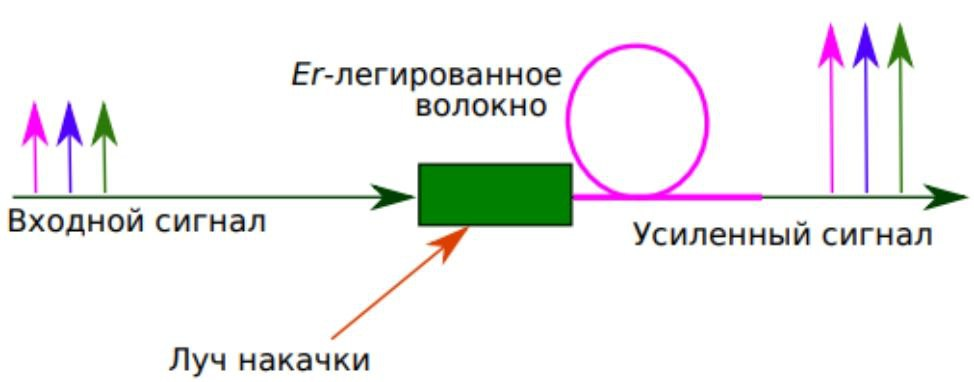
\includegraphics[width=0.60\linewidth]{erb_1.jpg}
		\caption{Схема волоконно-оптического усилителя}
		\label{labC}
	\end{figure}
	
	\begin{figure}[h!]
		\centering
		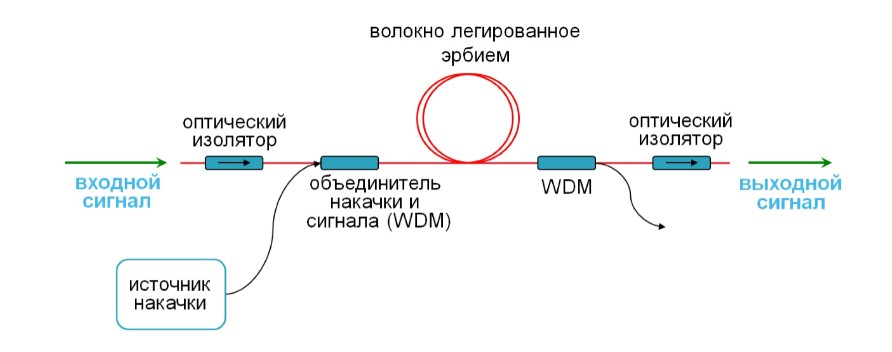
\includegraphics[width=0.80\linewidth]{erb_3.jpg}
		\caption{Схема волоконно-оптического усилителя}
		\label{lab}
	\end{figure}
		
Смешанный свет попадает в область волокна, легированную ионами
эрбия. Луч накачки передает свою энергию ионам эрбия, переводя их
внешние (оптические) электроны в возбуждённые состояния, создается
инверсная заселённость энергетических уровней эрбия. При поступлении
в систему фотона полезного (усиливаемого) сигнала, он, взаимодействуя с
возбуждённым атомом эрбия, вынуждает его излучить запасённую
энергию в виде дополнительного кванта излучения, свойства которого
идентичны свойствам изначального кванта полезного сигнала. Таким
образом, на каждый влетевший фотон полезного сигнала на выходе
образуется дополнительный когерентный фотон с такой же энергией,
фазой, поляризацией и направлением распространения – в этом и
заключается процесс увеличения интенсивности (усиления) входного
сигнала.

Среда с инверсной заселенностью является одной из главных
составных частей лазера, другой необходимой частью является система
оптической обратной связи, которая за счёт отражения возвращает часть
излучения обратно и тем самым создает непрерывную лазерную генерацию. Процесс непрерывной лазерной генерации превращает
усилитель в лазер и полностью нарушает структуру входного сигнала, что
препятствует передаче информации, поэтому от обратной оптической
связи стараются избавиться путём введения в систему оптических
«изоляторов» в тех местах, где обратная связь, обусловленная
отражением, может появляться: например на выходе из усилителя, в месте
присоединения к усилителю оптического волокна, которое представляет
собой границу раздела, на которой, ввиду механической неоднородности,
возникает отражение.
\begin{figure}[h!]
		\centering
		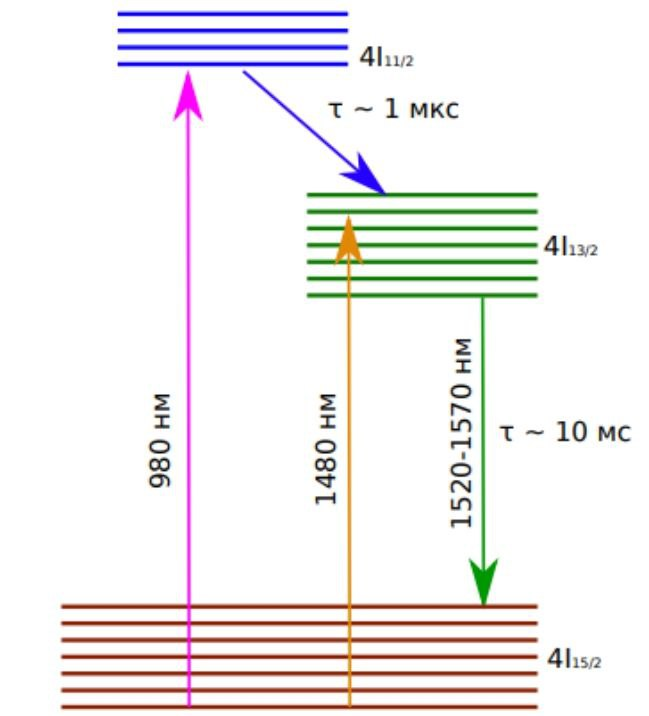
\includegraphics[width=0.60\linewidth]{levels.jpg}
		\caption{Схема энергетических уровней ионов  $Er^{3+}$ в кварцевом стекле}
		\label{labC}
	\end{figure}

 
 В процессе усиления в EDFA принимают участие уровни $4I_{13/2}$, $4I_{15/2}$ и
$4I_{11/2}$ Поглощение накачки на длине волны 980 нм переводит ионы $Er^{3+}$  из
основного состояния $4I_{15/2}$ на короткоживущий уровень $4I_{11/2}$, с которого в
процессе релаксации переходят на метастабильный уровень $4I_{13/2}$.
Уровень $4I_{13/2}$ называется метастабильным, поскольку время жизни частиц
в этом состоянии относительно велико (10 мс). Таким образом, даже
умеренный уровень мощности накачки позволяет перевести значительное
количество ионов эрбия в возбужденное состояние.

\subsubsection*{Исследование шум фактора}

Основным техническим параметром эрбиевого усилителя является коэффициент усиления. Коэффициент усиления G рассчитывается как отношение выходной мощности $P_{out}$ к входной $P_{in}$:

\begin{equation}
    G = \frac{P_{out}}{P_{in}}
\end{equation}

Для выражения коэффициента усиления в децибелах используется соотношение g = 10$\log G$. 

Помимо коэффициента усиления важной характеристикой оптического усилителя является шум-фактор, оценивающий степень ухудшения оптического отношения сигнал-шум (Optical Signal-to-NoiseRatio, OSNR) сигнала, который не содержит шумов вследствие прохождения через усилитель. Шум-фактор может выражаться как в линейных (F), так и в логарифмических единицах (NF = $10\log_{10}F$) и определяется соотношениями 
 	\begin{equation}
    F = \frac{OSNR_{in}}{OSNR_{out}}
 	\end{equation}
\begin{equation}
    NF = 10\log_{10}(\frac{OSNR_{in}}{OSNR_{out}}) = osnr_{in} - osnr_{out} 
\end{equation}
\begin{equation}    
    osnr_{out} = 10\log_{10}(OSNR_{out}) = p_{\Sigma} - p_{\text{сп}}
\end{equation}

где $p_{\Sigma}$ и $p_{\text{сп}}$ – суммарная мощность сигнала и спонтанного излучения и мощность спонтанного излучения в логарифмических единицах, соответственно (рис. 3).

\begin{figure}[h!]
		\centering
		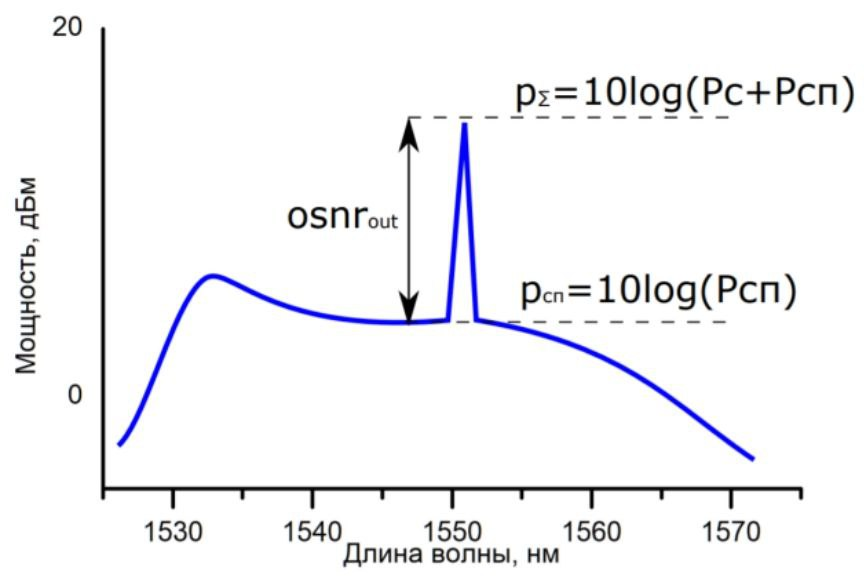
\includegraphics[width=0.5\linewidth, height=5.5cm]{erb-3.jpg}
		\caption{Спектральная зависимость усиления EDFA при различной выходной мощности.}
		\label{labC}
	\end{figure}

Оптическое отношение сигнал-шум принимает максимально возможное, так называемое квантово-ограниченное, значение отношения сигнал-шум:

\begin{equation*}
    OSNR_{in} = \frac{P_{in}}{h\nu\Delta \nu}
\end{equation*}

Таким образом, выражение для отношения сигнал-шум в линейных
единицах принимает следующий вид:

\begin{equation*}
    F = \frac{OSNR_{in}}{OSNR_{out}} = \frac{P_{S,in}}{h\nu\Delta \nu} \cdot \frac{1}{OSNR_{out}}
\end{equation*}

Переход в логарифмические единицы дает выражение:

\begin{equation*}
    NF = 10\log_{10}(F) = -10\log_{10}(h\nu\Delta \nu) + P_{S,in} - osnr_{out}
\end{equation*}

В частном случае на длине волны 1550 нм и в полосе 0,1 нм $10\log_{10}(h\nu\Delta \nu)$ = –51 дБм шум-фактор приобретает вид

\begin{equation*}
    NF = 51 + p_{S,in} - osnr_{out}
\end{equation*}

Эта формула позволяет измерить шум-фактор наиболее простым способом. Данная методика имеет ограничение – она применима только к лазерным сигналам, не содержащим шума усиленного спонтанного излучения.


\newpage
\section{Ход работы}

\subsection{Исследование спектра спонтанного усиленного
излучения.}

Для нескольких значений входной мощности измерили спектр спонтанно усиленного сигнала.

\begin{figure}[h!]
		\centering
		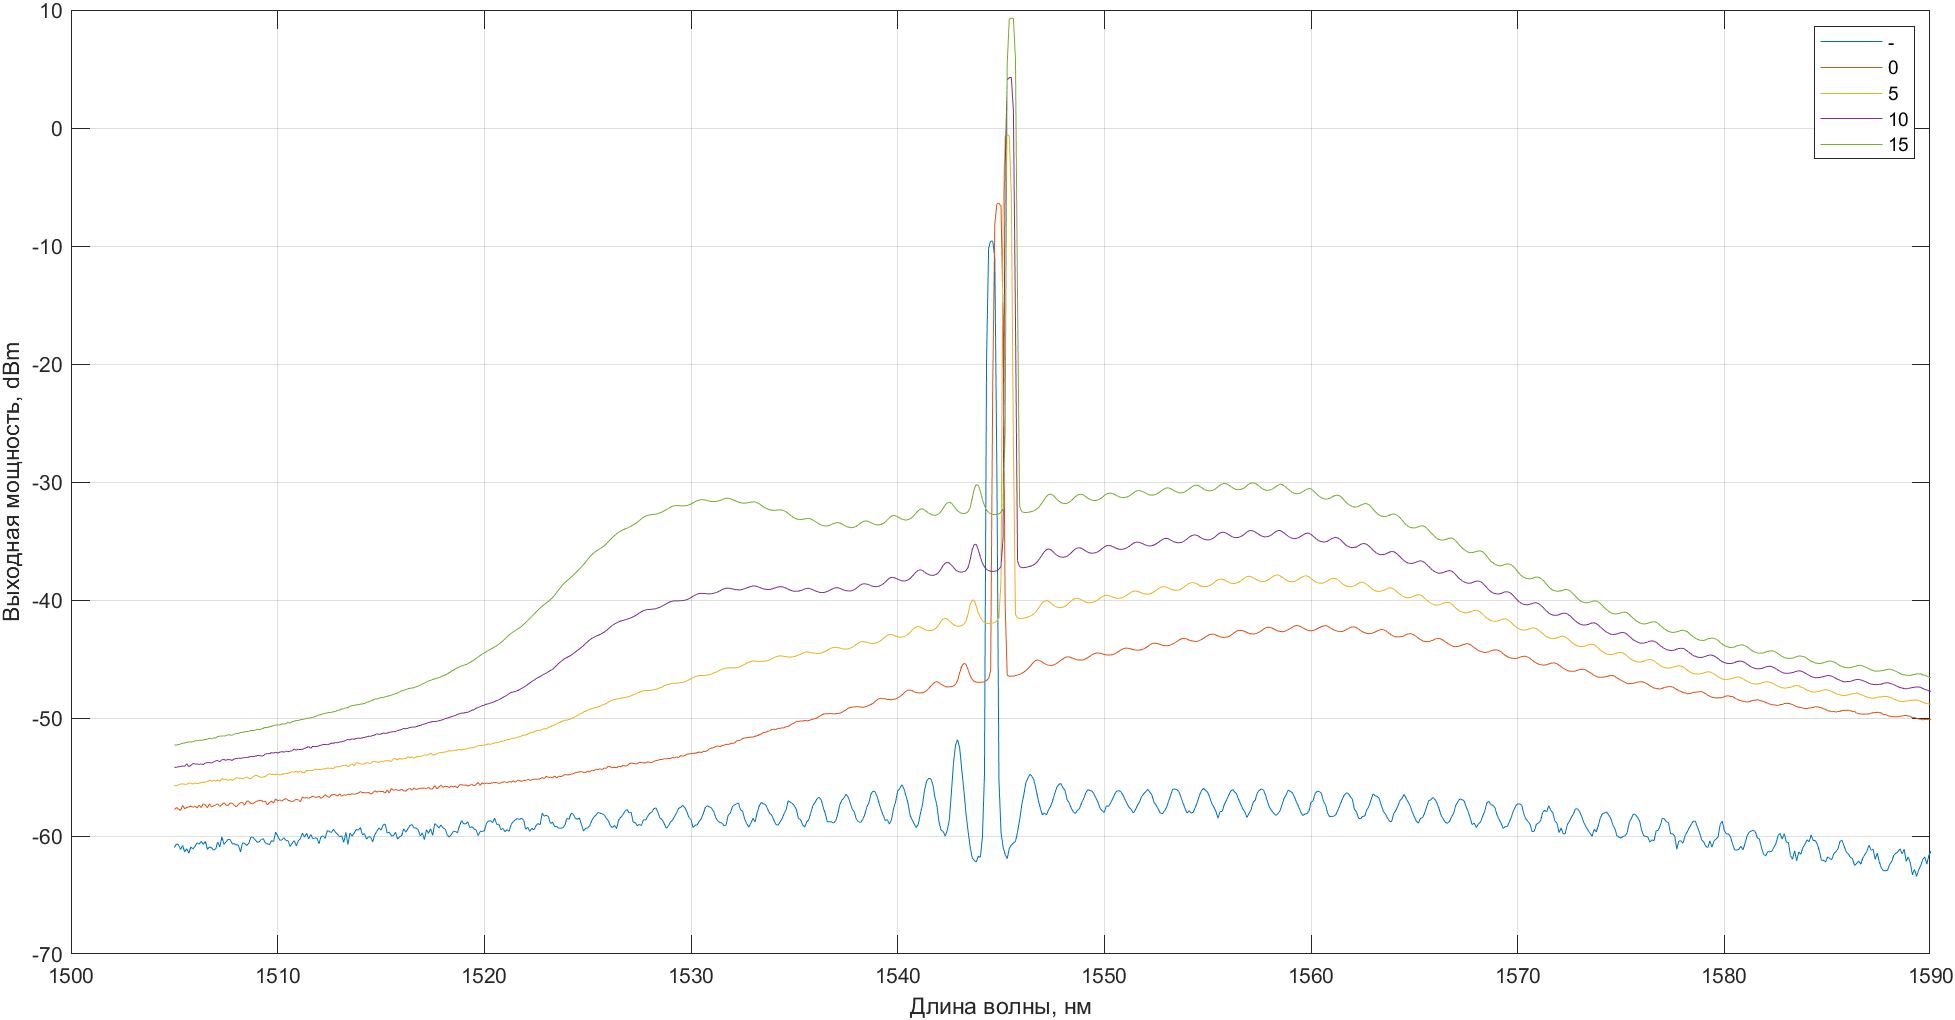
\includegraphics[width=0.99\linewidth]{point1.png}
		\caption{Спектральная зависимость усиления EDFA при различной выходной мощности.}
		\label{labC}
	\end{figure}

Сильный режим наблюдается на уровне 1545 нм.
В этом спектральном диапазоне ненакачанное волокно показывает существенные потери, но высокое усиление. 

Рассчитаем величину шум-фактора при различных значениях выходной мощности в логарифмических единицах:

\begin{center}
\begin{tabular}{|c|c|}
    \hline
    $P_in$, dBm & NF, dBm \\
     \hline
     0 & -33 \\
     \hline
     5 & -31 \\
     \hline
     10 & -24 \\
     \hline
     15 &  -23 \\
     \hline
\end{tabular}
\end{center}

\newpage
 
\subsection{Зависимость выходной мощности EDFA от тока накачки.}
Включаем источник излучения на длине волны 1545 нм,измеряем мощность входного излучения.Включаем лазер накачки.Измеряем мощность накачки. На графике представлена полученная зависимость входной мощности на максимально возможное значения для усилителя при увеличении тока накачки

\begin{figure}[h!]
		\centering
		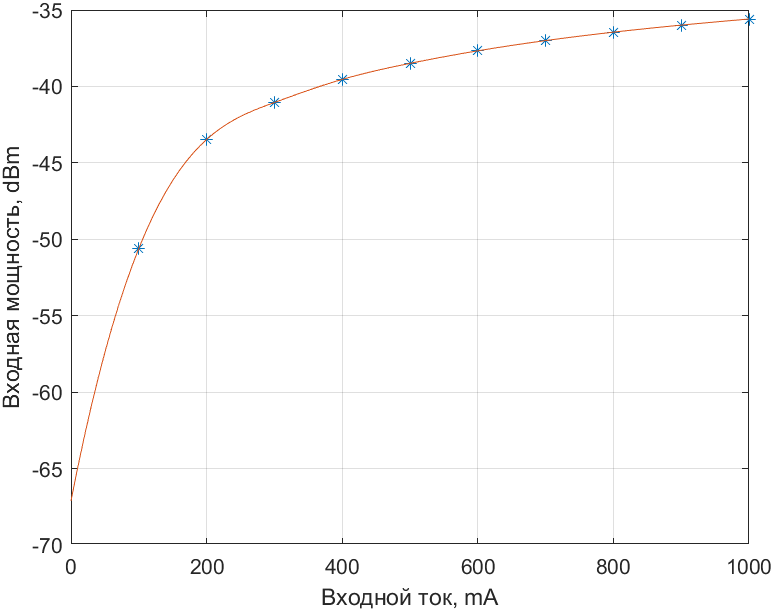
\includegraphics[width=0.6\linewidth, height=8cm]{point3.png}
		\caption{Зависимость выходной мощности от тока накачки}
		\label{labC}
	\end{figure}
	
	
Исследуем зависимость выходной мощности EDFA от тока накачки и входной мощности для трёх значений токов накачки I = 0, 50, 90 mA.По полученному набору значений построим график коэффициента усиления от входной мощности.

\begin{figure}[h!]
    \begin{center}
    \begin{minipage}[h!]{0.49\linewidth}
    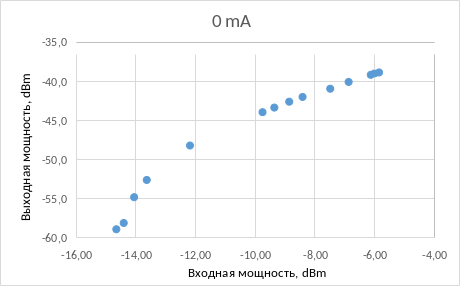
\includegraphics[width = 1\textwidth]{point_4_0.png}
    \caption{Вых./вх. мощность I = 0 mA}
    \label{1}
    \end{minipage}
    \begin{minipage}[h!]{0.49\linewidth}
    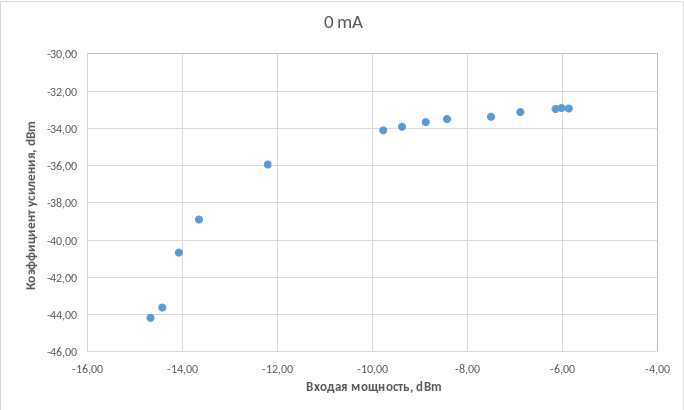
\includegraphics[width = 1\textwidth]{point5_0.png}
    \caption{Коэфф. усиления от вх. мощности}
    \label{2}
    \end{minipage}
    \end{center}
\end{figure}  

\begin{figure}[h!]
    \begin{center}
    \begin{minipage}[h!]{0.49\linewidth}
    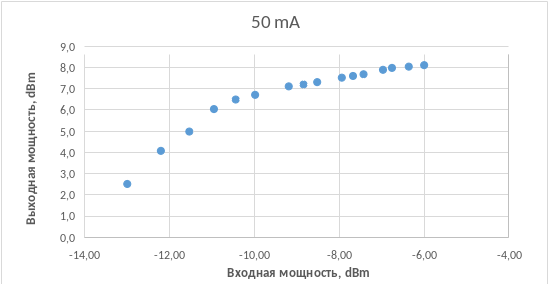
\includegraphics[width = 1\textwidth, height=7cm]{point_4_50.png}
    \caption{Вых./вх. мощность I = 50 mA}
    \label{1}
    \end{minipage}
    \begin{minipage}[h!]{0.49\linewidth}
    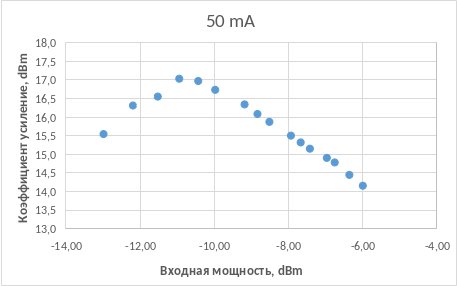
\includegraphics[width = 1\textwidth, height=7cm]{point_5_50.png}
    \caption{Коэфф. усиления от вх. мощности}
    \label{2}
    \end{minipage}
    \end{center}
\end{figure}  

\begin{figure}[h!]
    \begin{center}
    \begin{minipage}[h!]{0.49\linewidth}
    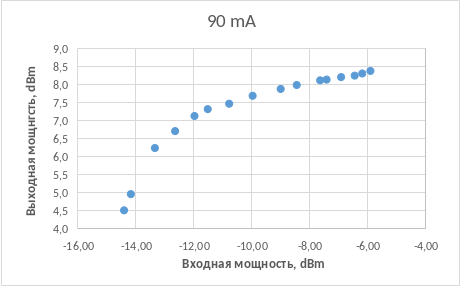
\includegraphics[width = 1\textwidth, height=7cm]{point_4_90.png}
    \caption{Вых/вх. мощность I = 90}
    \label{1}
    \end{minipage}
    \begin{minipage}[h!]{0.49\linewidth}
    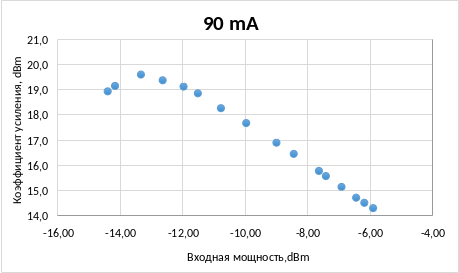
\includegraphics[width = 1\textwidth, height=7cm]{point_5_90.png}
    \caption{Коэфф. усиления от вх. мощности}
    \label{2}
    \end{minipage}
    \end{center}
\end{figure}  

\begin{figure}[h!]
		\centering
		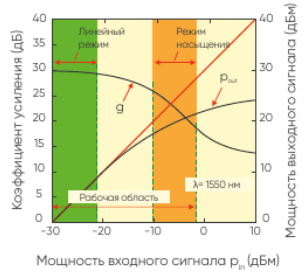
\includegraphics[width=0.5\linewidth, height=6.5cm]{point5_th.png}
		\caption{График теоретических зависимостей к пункту 2.3}
		\label{labC}
\end{figure}

\newpage

\section{Приложение. Таблицы экспериментальных значений}

\begin{tabular}{|c|c|c|c|c|c|c|c|c|}
\hline 
\multicolumn{9}{|c|}{I = 0 mA}  \\ 
\hline 
$P_{in}$, dBm & -14.69 & -14.44 & -14.09 & -13.67 & -12.22 & -7.52 & -5.88 & -6.04  \\ 
\hline 
$P_{out}$, dBm & -58.8 & -58.0 & -54.7 & -52.5 & -48.1 & -40.84 & -38.79 & -38.89  \\ 
\hline 
g, dBm & -44.11 & -43.56 & -40.61 & -38.83 & -35.88 & -33.32 & -32.88 & -32.85 \\ 
\hline 
$P_{in}$, dBm & -6.16 & -6.90 & -9.79 & -9.39 & -8.89 & -8.45 & • & • \\ 
\hline 
$P_{out}$, dBm & -39.06 & -39.97 & -43.84 & -43.25 & -42.50 & -41.89 & • & • \\ 
\hline 
g, dBm & -32.90 & -33.07 & -34.05 & -33.86 & -33.61 & -33.44 & • & • \\ 
\hline 
\multicolumn{9}{|c|}{I = 90 mA}\\ 
\hline 
$P_{in}$, dBm & -5.93 & -6.22 & -6.48 & -6.95 & -7.45 & -7.67 & -8.48 & -9.03 \\ 
\hline 
$P_{out}$, dBm & 8.41 & 8.34 & 8.28 & 8.24 & 8.17 & 8.15 & 8.02 & 7.91 \\ 
\hline 
g, dBm & 14.34 & 14.56 & 14.76 & 15.19 & 15.62 & 15.82 & 16.50 & 16.94 \\ 
\hline 
$P_{in}$, dBm &  -10.00 & -10.81 & -11.55 & -12.01 & -12.68 & -13.37 & -14.20 & -14.44 \\ 
\hline 
$P_{out}$, dBm & 7.72 & 7.50 & 7.35 & 7.16 & 6.74 & 6.27 & 4.99 & 4.54 \\ 
\hline 
g, dBm & 17.72 & 18.31 & 18.90 & 19.17 & 19.42 & 19.64 & 19.19 & 18.98 \\ 
\hline 
\multicolumn{9}{|c|}{I = 50 mA} \\ 
\hline 
$P_{in}$, dBm & -6.02 & -6.38 & -6.78 & -6.99 & -7.45 & -7.70 & -7.96 & -8.54  \\ 
\hline 
$P_{out}$, dBm & 8.16 & 8.09 & 8.03 & 7.94 & 7.73 & 7.65 & 7.57 & 7.36 \\ 
\hline 
g, dBm & 14.18 & 14.47 & 14.81 & 14.93 & 15.18 & 15.35 & 15.53 & 15.90  \\ 
\hline 
$P_{in}$, dBm & -8.86 & -9.21 & -10.00 & -10.45 & -10.97 & -11.55 & -12.22 & • \\ 
\hline 
$P_{out}$, dBm & 7.25 & 7.16 & 6.76 & 6.54 & 6.09 & 5.03 & 4.12 & • \\ 
\hline 
g, dBm & 16.11 & 16.37 & 16.76 & 17.00 & 17.06 & 16.58 & 16.34 & • \\ 
\hline 
\end{tabular} 

\end{document}
